\documentstyle[11pt,epsfig,fancybox,semcolor,semlayer,doublespace,portrait]
{seminar}
\input clp_utils

\def\lep{{\sc Lep}}
\def\aleph{{\sc Aleph}}
\def\lthree{{\sc L3}}
\def\cdf{{\sc Cdf}}
\def\dzero{{\sc D0}}
\def\slac{{\sc Slac}}
\def\sld{{\sc Sld}}
\def\lhc{{\sc Lhc}}
\def\qqbar{q\={q}}
\def\ccbar{c\={c}}
\def\bbbar{b\={b}}
\def\ttbar{t\={t}}
\def\inv{$^{\mbox{\scriptsize -1}}$}

\newcommand{\talktitle}[0]{Ritchie's Question}
\newcommand{\fmttitle}[0]{}
\newcommand{\conftitle}[0]{A Exam}
\newcommand{\myname}[0]{Jim Pivarski}
\newcommand{\affila}[0]{Cornell University}
\newcommand{\talkdate}[0]{October 3, 2002}

\pagestyle{conference}   % From clp_utils.tex

% slide magnification
\slidesmag 1

%%%%%%%%%%%%%%%%%%%%%%%%%%%%%%%%%%%%%%%%%%%%%%%%%%%%%%%%%%%%%%%%%%%%%%%%%%%
% Start document
\begin{document}

% Set page size
\slideheight 7.0in
\slidewidth 8.8in 

% Set array stretch
\renewcommand{\arraystretch}{0.3}
\renewcommand{\slidetopmargin}{0.4in}
\renewcommand{\slidebottommargin}{0.9in}


%%%%%%%%%%%%%%%%%%%%%%%%%%%%%%%%%%%%%%%%%%%%%%%%%%%%%%%%%%%%%%%%%%%%%%%%%%%

% %%%%%%%%%%%%%%%%%%%%%%%%%%%%%%%%%%%%%%%%%%%%%%%%%%%%%%%%%%%%%%%%%%%%%%%%%%%

% \begin{slide*}

% \slideframe{}
% \slideframe*[\dkblue]{Oval}
% \huge
% \heading{Outline}
% \vspace{1 cm}

% \begin{center}
% \begin{minipage}[t]{12 cm}
% \begin{itemize}
% \LARGE \item {\huge Motivation: verify lattice QCD!}
% \LARGE \item {\huge 2 out of 3 Resonances Scanned}
% \LARGE \item {\huge Energy Calibration Systematics}
% \LARGE \item {\huge Other Systematics / Work to be Done}
% \end{itemize}
% \end{minipage}
% \end{center}

% \end{slide*}
 
%%%%%%%%%%%%%%%%%%%%%%%%%%%%%%%%%%%%%%%%%%%%%%%%%%%%%%%%%%%%%%%%%%%%%%%%%%%

\begin{slide*}

\slideframe{}
\slideframe*[\dkblue]{Oval}

\begin{center}
  \begin{tabular}[t]{c p{0.25cm} c}
    \includegraphics[scale=0.5]{production_gluon_fusion.eps} & &
    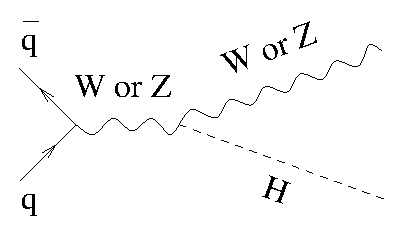
\includegraphics[scale=0.5]{production_higgsstrahlung.eps} \\
    {\bf Gluon Fusion} (gg $\to$ h$_{\mbox{\scriptsize SM}}$) & &
    {\bf Higgsstrahlung} (\qqbar\ $\to$ h$_{\mbox{\scriptsize SM}}$\{W,Z\}) \\
    & \vspace{0.25cm} & \\
    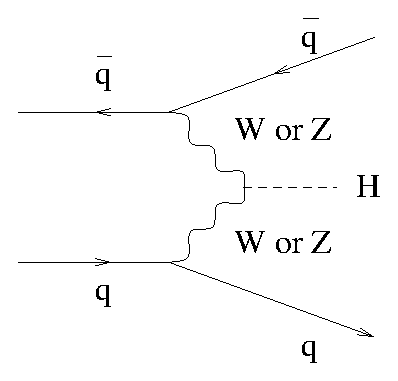
\includegraphics[scale=0.5]{production_vector_boson_fusion.eps} & &
    \includegraphics[scale=0.5]{production_tt_fusion.eps} \\
    {\bf Vector Boson Fusion} (\qqbar\ $\to$ h$_{\mbox{\scriptsize SM}}$\qqbar) & &
    {\bf \ttbar\ Fusion} (gg $\to$ h$_{\mbox{\scriptsize SM}}$\ttbar) \\
  \end{tabular}
\end{center}

\begin{center}
  \includegraphics[width=0.9\linewidth]{higgs_production.eps}
\end{center}

\end{slide*}

%%%%%%%%%%%%%%%%%%%%%%%%%%%%%%%%%%%%%%%%%%%%%%%%%%%%%%%%%%%%%%%%%%%%%%%%%%%

\begin{slide*}

\slideframe{}
\slideframe*[\dkblue]{Oval}

\begin{center}
  \begin{tabular}{c p{0.25cm} c}
    \includegraphics[height=7cm]{s02_mw.eps} & &
    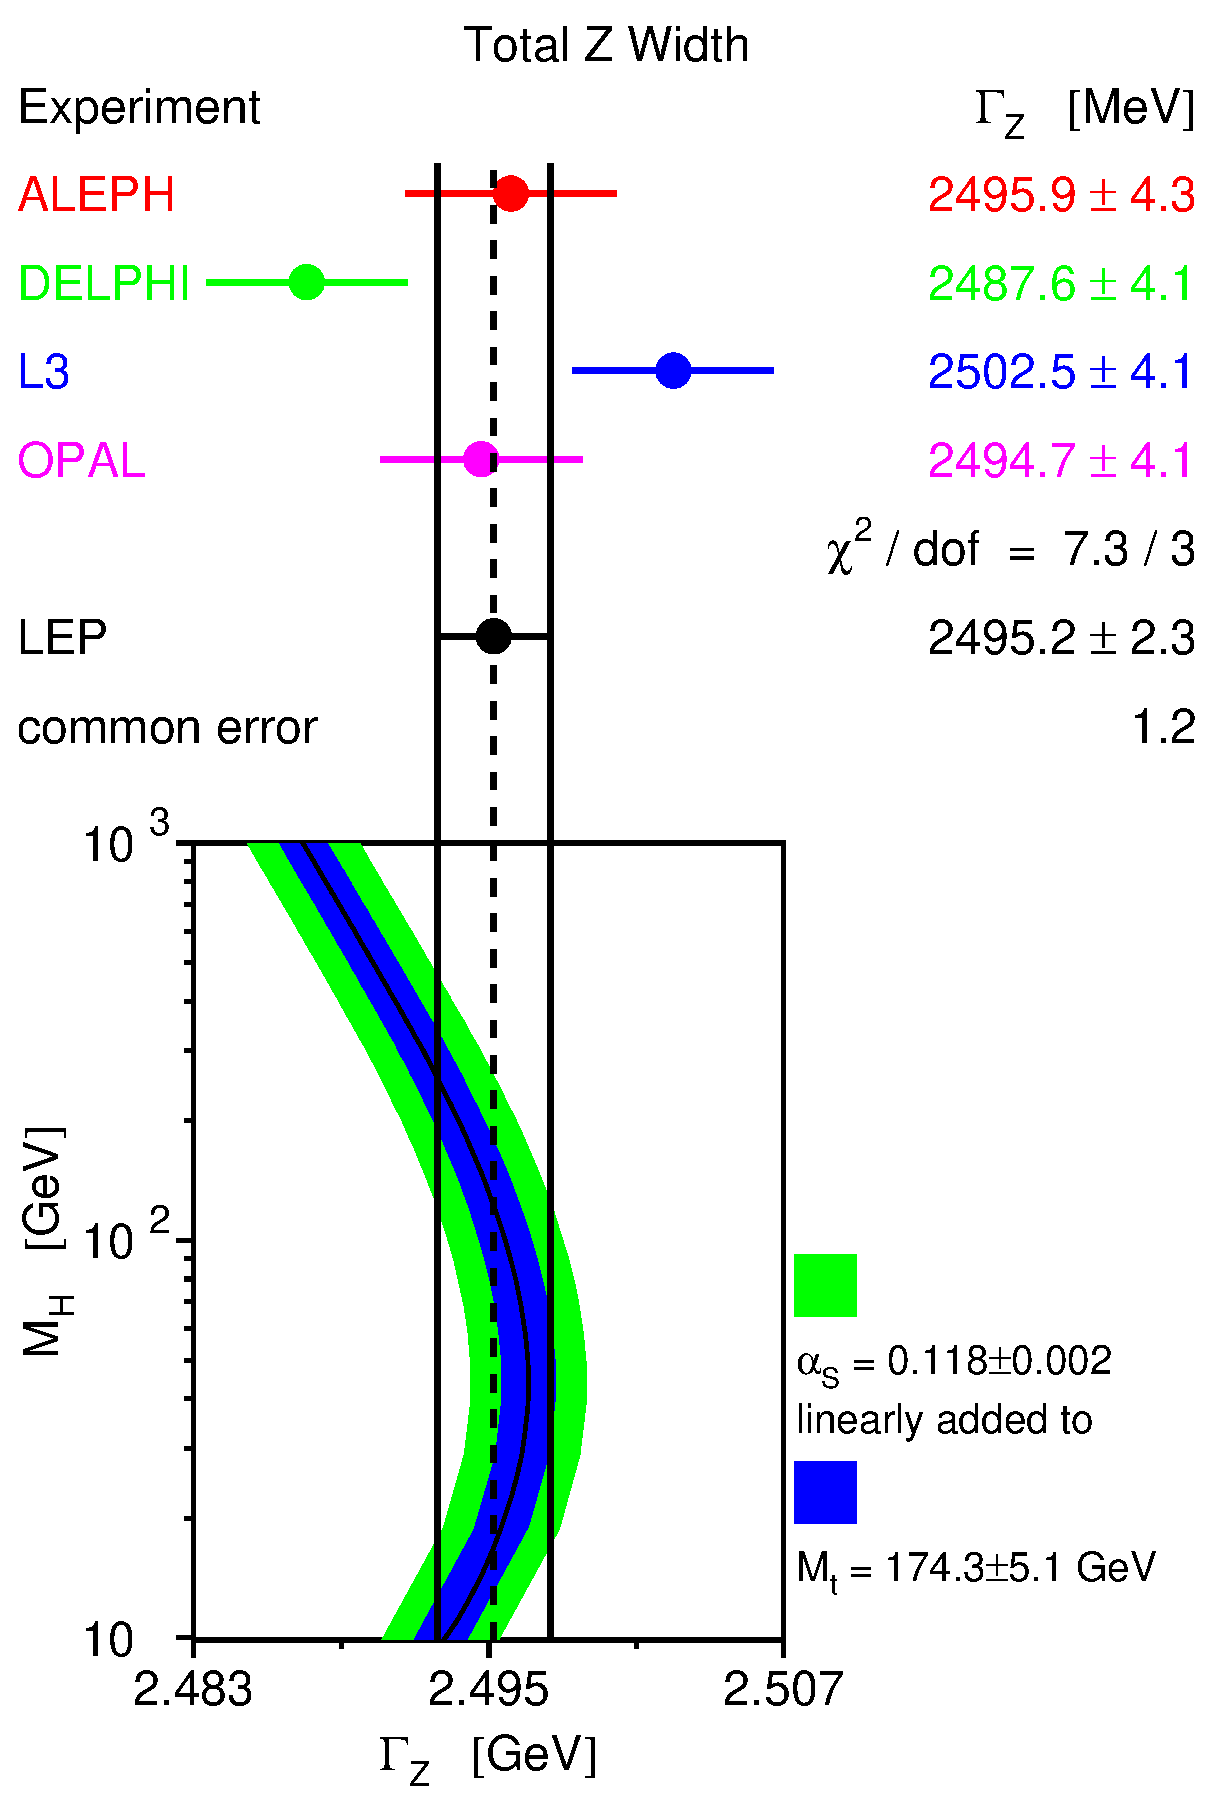
\includegraphics[height=7cm]{lep1_gz.eps} \\
    {\bf Mass of the W Boson (\lep)} & & {\bf Width of the Z Boson (\lep)} \\
    & \vspace{0.25cm} & \\
    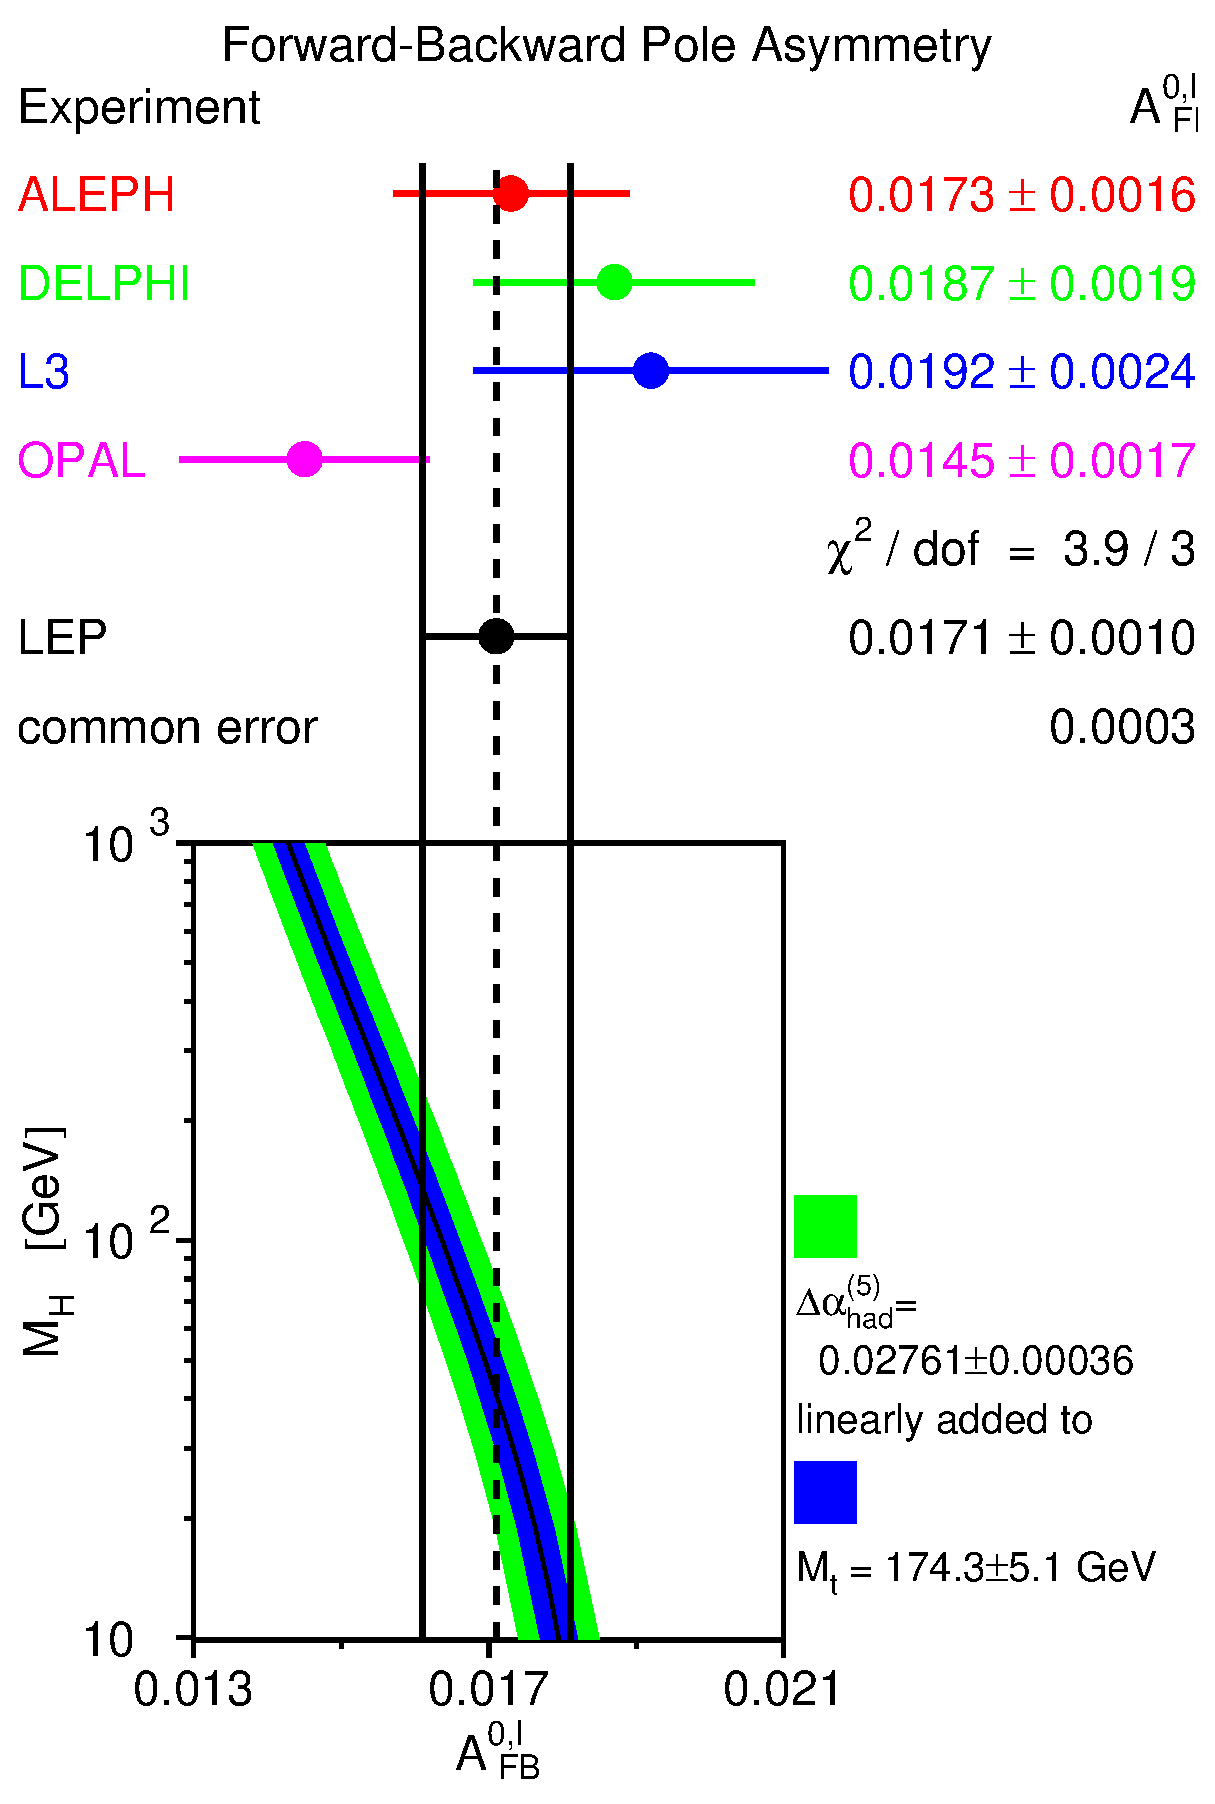
\includegraphics[height=7cm]{lep1_al.eps} & &
    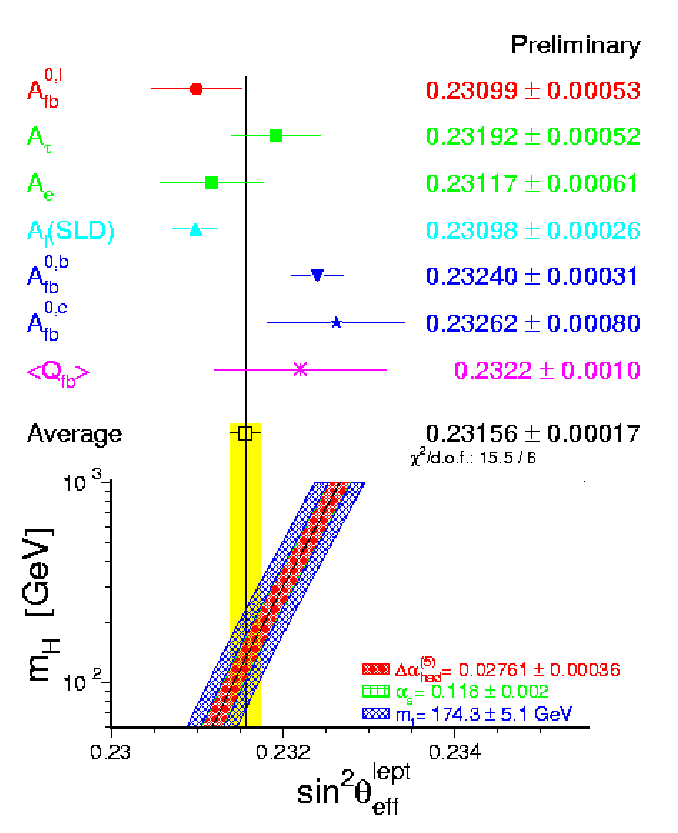
\includegraphics[height=7cm]{sld_al.eps} \\
    {\bf Z-Pole Asymmetry (\lep)} & & {\bf Weak Mixing Angle (\sld)} \\
  \end{tabular}
\end{center}

\end{slide*}

%%%%%%%%%%%%%%%%%%%%%%%%%%%%%%%%%%%%%%%%%%%%%%%%%%%%%%%%%%%%%%%%%%%%%%%%%%%

\begin{slide*}

\slideframe{}
\slideframe*[\dkblue]{Oval}

\begin{center}
  \vfill
  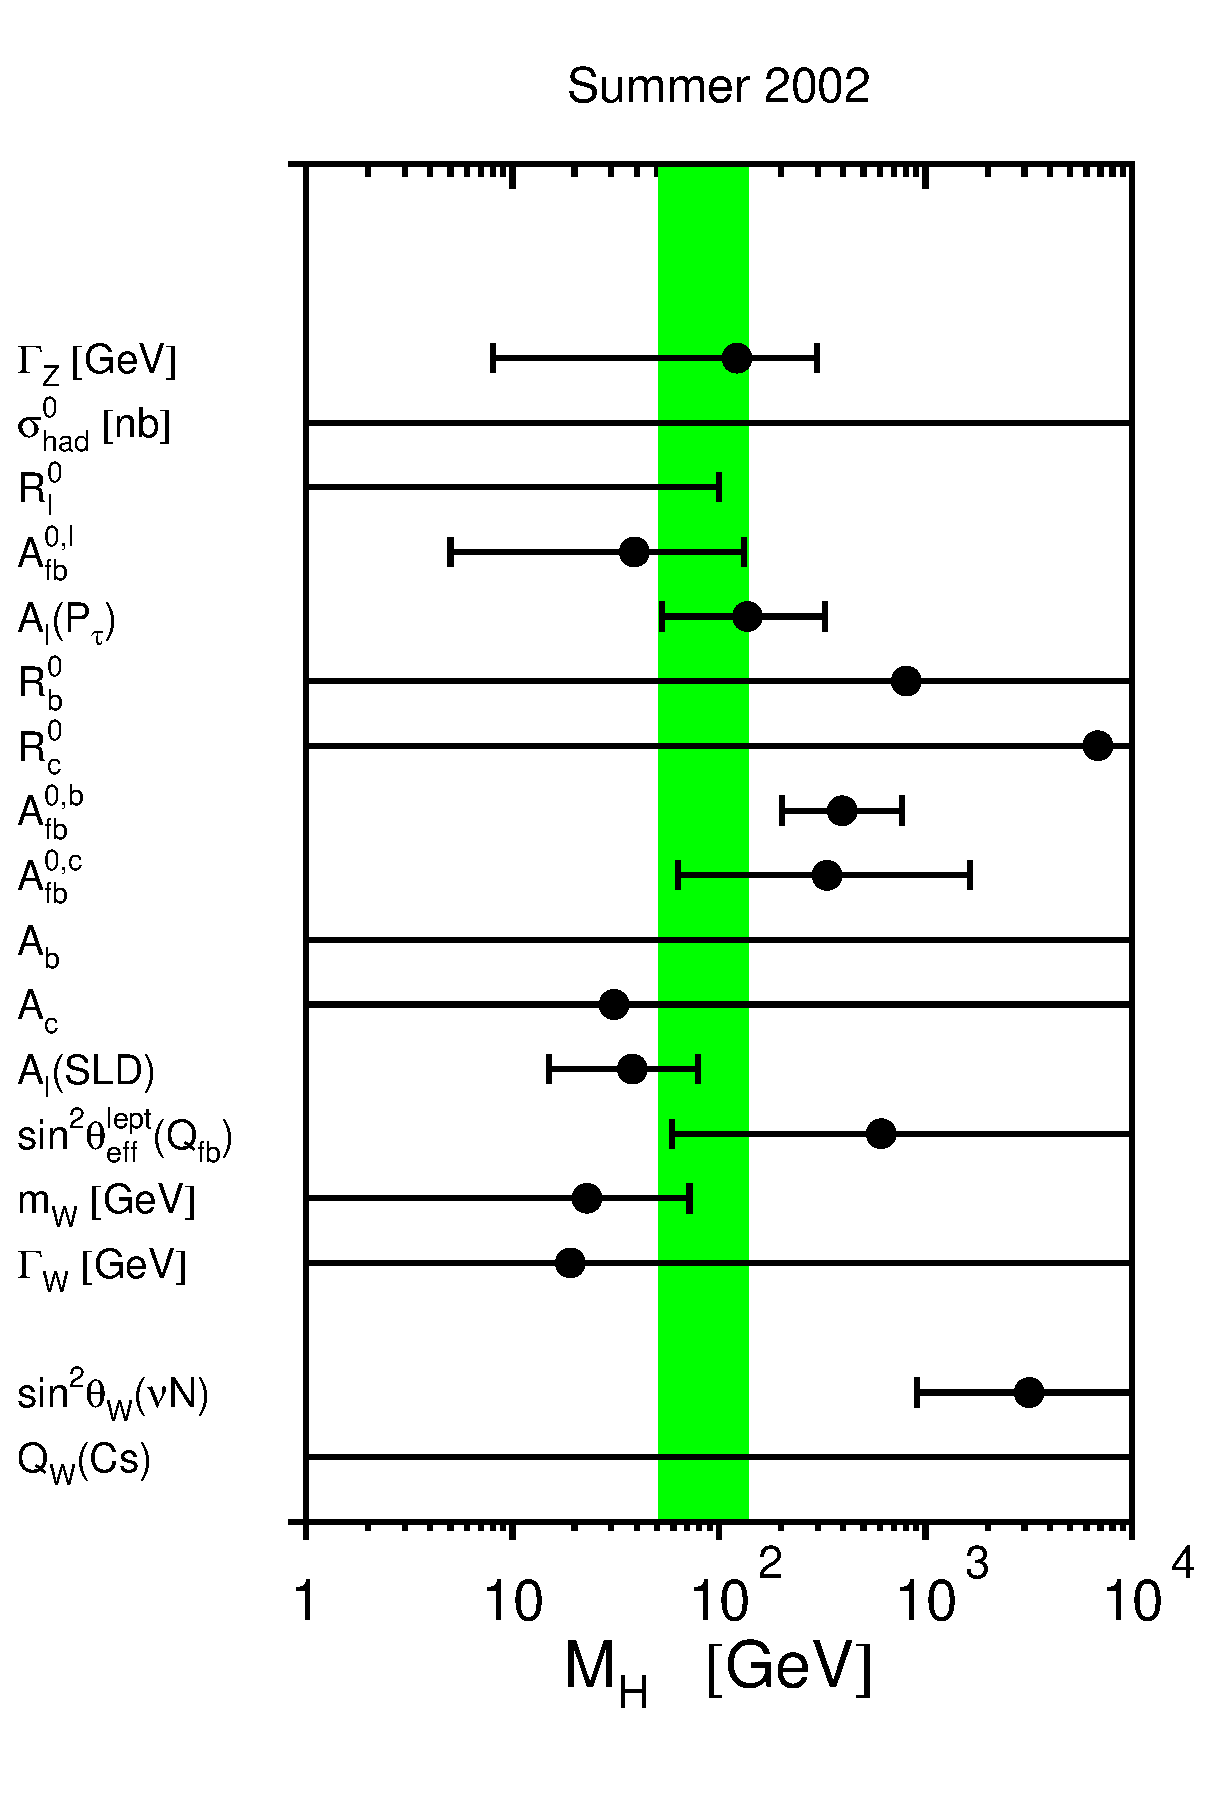
\includegraphics[height=11cm,angle=-90]{s02_show_higgs.eps} \\
  \vfill
  \includegraphics[height=11cm,angle=-90]{mass_pdf.eps}
  \vfill
\end{center}

\end{slide*}

%%%%%%%%%%%%%%%%%%%%%%%%%%%%%%%%%%%%%%%%%%%%%%%%%%%%%%%%%%%%%%%%%%%%%%%%%%%

\begin{slide*}

\slideframe{}
\slideframe*[\dkblue]{Oval}

\begin{center}
  \vfill

  {\bf Tevatron Signatures} \\
  \begin{tabular}[t]{c p{0.25cm} c}
    \includegraphics[scale=0.5]{signature_LA.eps} & &
    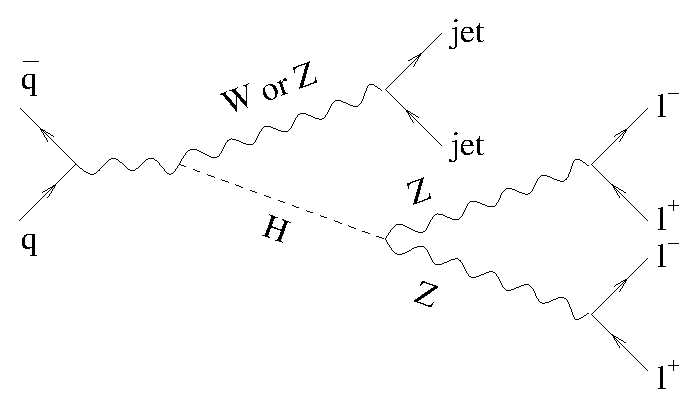
\includegraphics[scale=0.5]{signature_HB.eps} \\
    $\ell \nu \mbox{b\={b}}$, $\nu \bar{\nu} \mbox{b\={b}}$ and $\ell^+ \ell^- \mbox{b\={b}}$ & &
    $\ell^\pm \ell^\pm$ jet jet \\
    & \vspace{0.25cm} & \\
    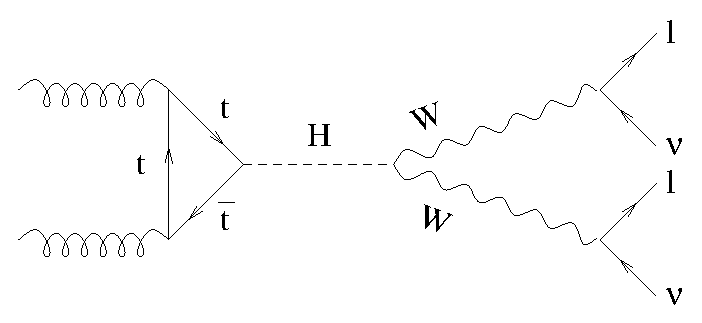
\includegraphics[scale=0.5]{signature_HC.eps} & &
    \includegraphics[scale=0.5]{signature_HB2.eps} \\
    $\ell \bar{\nu} \bar{\ell} \nu$ & &
    $\ell^\pm \ell^\pm$ jet jet \\
  \end{tabular}

  \vfill

  {\bf \lhc\ Signatures} \\
  \begin{tabular}[t]{c p{0.25cm} c}
    \includegraphics[scale=0.5]{signature_LB_correct.eps} & &
    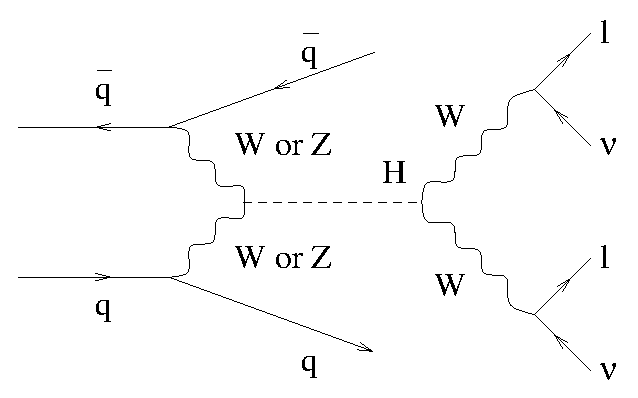
\includegraphics[scale=0.5]{signature_HA_correct.eps} \\
    $\ell^+ \bar{\nu} \nu \, \ell^- \nu \bar{\nu}$ + 2 forward jets & &
    $\ell \bar{\nu} \bar{\ell} \nu$ + two forward jets \\
  \end{tabular}

  \vfill
\end{center}

\end{slide*}

%%%%%%%%%%%%%%%%%%%%%%%%%%%%%%%%%%%%%%%%%%%%%%%%%%%%%%%%%%%%%%%%%%%%%%%%%%%

\end{document}

% %%%%%%%%%%%%%%%%%%%%%%%%%%%%%%%%%%%%%%%%%%%%%%%%%%%%%%%%%%%%%%%%%%%%%%%%%%%

% \begin{slide*}

% \slideframe{}
% \slideframe*[\dkblue]{Oval}
% \huge
% \heading{}

% \begin{minipage}[t]{\linewidth}

% \end{minipage}

% \end{slide*}


